\documentclass[catalan,11pt,a4paper]{report}
%Per a que els titols surtin en català.
\usepackage[catalan]{babel}
%Per a poder escriure accents
\usepackage[utf8]{inputenc}
%Per a poder incloure grafics
\usepackage{graphicx}
\usepackage{url}
%Incorpora enllaços a referencies (colorlinks=true canvia el text dels enllaços)
\usepackage[colorlinks=false]{hyperref}  %incorpora enllaços a referències, seccions i url's. També genera índex pdf

%%%%%% Estructura de la pagina %%%%
\setlength{\parskip}{1.7ex plus 0.5ex minus 0.5ex}
\setlength{\parindent}{1.3em}

\author{Sergi Almacellas Abellana}
\title{Implementació de la Botifarra utilitzant WebSockets, HTML5 i Javascript}

\begin{document}
\begin{titlepage}
\begin{center} 


\includegraphics{img/M-UdL_rs.png}

{\fontfamily{ptm}\selectfont\Large Escola Politècnica Superior}\\[1.5cm]   %ptm: Times font (UdL corporatiu)
\Large Màster en Enginyeria de Programari Lliure\\[3mm]
\textsc{\LARGE Treball de Final de Màster}\\[1.5cm]

\rule{\linewidth}{1.5pt} \\[7mm]

{\huge \bf Implementació de la Botifarra utilitzant WebSocket, HTML5 i Javascript } \\[2mm]
\rule{\linewidth}{1.5pt} \\[1cm]
\large
\begin{minipage}{0.49\textwidth}
\textsl{Autor:}\\Sergi Alamcellas Abellana
\end{minipage}
\begin{minipage}{0.49\textwidth}\begin{flushright}
\textsl{Director:}\\Juan Manuel Gimeno Illa 
\end{flushright}\end{minipage}

\vfill\today

\end{center}
\end{titlepage}

\tableofcontents
\newpage
\chapter*{Agraiments}
\addcontentsline{toc}{chapter}{Agraiments}

Aquest projecte no hagues estat possible sense l'ajuda de moltes persones. Per aquest motiu m'agradaría dedicar unes línies a cadascun d'ells per agraïr-los la seva ajuda.

Primer de tot vuldría agraïr a tota la meua família pel seu recolzament (en aquest i altres projectes) i per la seva ajuda a prioritzar projecte, especialment per recordar-m'he que aquest era dels més prioritaris. 

També m'agradaría agrair a Juan Manuel Gimeno Illa, qui em va proposar la idea d'aquest projecte, per la seva ajuda en el desenvolupament i per accepart-m'he com a projectista. 

També agrair l'ajuda pel que fa la documentació a Gerard Bosch Montserrate, especialment per compartir els seus coneixements de LaTeX.

També agraïr a Pedro Teixeira el desenvolupament de la web Nodetuts.org, on es poden trobar petits tutorials en forma de vídeo del funcionament de Node.

Finalment, un agraïment per aquells que s'han interesat pel projecte i pels que han ajudat al desenvolupament del mateix, ja sigui donant idees o provan el funcionament del projecte. 


%\chapter*{Llicència}
\addcontentsline{toc}{chapter}{Llicència}

Aquesta memòria està llicenciada sota la llicència lliure Creative Commons CC-BY-NC-SA. Podeu trobar una copia complerta de la llicència a \url{http://creativecommons.org/licenses/by-nc-sa/3.0/legalcode}

Aquesta llicència us permet: 

\begin{itemize}
    \item{Copiar i destribuir el document}
    \item{Modificar i redistribuir la totalitat o part d'aquest document}
    \item{Fer ús comercial de la totalitat o part d'aquest document} 
\end{itemize}

Sempre que respecteu les següents condicions: 

\begin{itemize}
    \item{Citar l'autor d'aquest document com a font del vostre treball}
    \item{Redistribuir el treballa sota la mateixa llicència o una similar}
\end{itemize}

Podeu trobar una còpia del codi font d'aquest document a \url{https://github.com/pokoli/memory}


\chapter{Introduccio}

El projecte consisteix en implementar una versió multi-jugador del Joc de la Botifarra. Aquest joc no ha de necesitar la instal·lació de cap software especific, sinó que ha de ser accessible a través de qualsevol navegador web modern.

\section{El perquè de tot plegat}

\section{Objectius}
L'objectiu principal d'aquest projecte es la presa de contacte amb noves tecnologies. Al capítol \ref{sec:tecnologies} es detalla més profundament quines tecnologies s'han utilitzat durant el projecte i perquè s'han utilitzat aquestes i no unes altres. 

Per tal de posar en joc totes aquestes tecnologies el JM em va proposar crear un joc en línia. Ell em va proposar crear un domino o un parxís. Degut al meu fanatisme per la botifarra i que feia molts dies que havia pensat en crear un joc així, vaig proposar de realitzar un joc de la botifarra, que és el que finalment s'ha realitzat. 

Personalment vaig posar un objectiu addicional al projecte: Utilitzar el Test Driven Development per tal de poder veure amb primera persona com funciona, i descobrir les ventatges i inconvenients que té usar-lo. 

Com a altres objectius del projecte podem nombrar els següents: 
\begin{itemize}
	\item{Tenir contacte amb altres usuaris de la comunitat internacional que estiguin implicats amb projectes similars.}
	\item{Aprendre a utilitzar forges per a compartir codi (i informació relacionada amb el mateix) amb altres usuaris.}
\end{itemize} 

Aquest objectius venen implícits en el mateix projecte degut a que aquest s'està desenvolupant en el Màster amb Enginyeria del Programari Lliure. 




\chapter{Requeriments del sistema}

Es vol construir un sistema que sigui capas de allotjar jocs en linia a través d'un navegador. 
Aquest sistema ha d'utilizar la teconologia client-servidor, es a dir hi ha d'haver un programa servidor que es l'encarregat d'allotjar les dades de totes les partides i un programa client que és l'encarregat de mostrar a l'usuari totes aquestes dades. 
 

\section{Funcions del servidor}

El programa servidor ha de realitzar les següents tasques:

\begin{enumerate}
	\item{Acceptar conexions per part dels clients.}
	\item{Comunicarse amb els clients de forma bidireccional, és a dir, ha de ser capaç d'enviar dades als clients  i també rebre'n dades.}
	\item{Allotjar diferents partides de forma simultánea.}
	\item{Proporcionar mecanismes necesaris perque els clients poguin crear partides i veure les que han estat creades per altres usuaris.}
	\item{Notificar als clients de tots els events que es produeixen en el joc que estan jugant.}
	\item{Permetre la comunicació entre els diferents clients connectats al servidor}	
\end{enumerate}

\section{Funcions del client}

El programa client ha de realitzar les següents tasques: 

\begin{enumerate}
	\item{Permtere a l'usuari communicarse amb el servidor de jocs.}
	\item{Rebre informació del programa servidor i mostrar-la a l'usuari d'una forma amigable.}
	\item{Interactuar amb l'usuari per tal de proporcionar al programa servidor la informació que aquest sol·liciti.}	
\end{enumerate}



\chapter{La botifarra}
\label{chap:botifarra}

En aquesta secció es descriurà com funciona el Joc de la botifarra i les seves regles. A part també es descriuran els aspectes a tenir en compte de cara al programa. 


El joc es juga entre quatre jugadors, que formant parella, seuran l'un al davant de l'altre. S'utilitza una baralla de 48 cartes formada per quatre colls (oros, copes, espases i bastos) amb 12 cartes cadascun, altrament coneguda com la baralla espanyola.


L'objectiu de la partida és superar els 100 punts abans que la parella contrària. 


\section{Puntuació}

El valor de cadascuna de les cartes és:
\begin{itemize}
	\item{Manilla (9), 5 punts}
    \item{As (1), 4 punts}
    \item{Rei (12), 3 punts}
    \item{Cavall (11), 2 punts}
    \item{Sota (10), 1 punt}
\end{itemize}

La resta de cartes no tenen cap punt.
    
Dins d'un mateix coll, l'ordre de les cartes de més alta a més baixa és el següent: 9, 1, 12, 11, 10, 8, 7, 6, 5, 4, 3 i 2.

Per cada basa\footnote{Una basa està formada per 4 cartes que ja s'han jugat.} guanyada es compta un punt. Això vol dir que en cada mà o dat hi ha 72 punts a repartir entre les dues parelles.

La parella guanyadora de cada mà, s'apuntarà la quantitat de punts que passi de 36. Aquest resultat s'haurà de doblar si el trumfo és botifarra. Cal tenir en compte que aquesta quantitat s'haurà de multiplicar en funció de si algún jugador ha vulgut augmentar el valor de la ronda. Per augmentar el valor de la partida s'utilitzen les paraules: \emph{contro}, \emph{recontro} i \emph{Sant Vicenç}. A la secció \ref{sec:contros} s'explica com un jugador pot augmentar el valor de la ronda.

\section{Mecànica de joc}

El joc de la botifarra es composa per un nombre variables de rondes. De cada ronda es computa la puntuació tal com s'ha comentat a l'apartat anterior. Així, es van jugant rondes fins que un dels dos equips es proclama guanyador.

\subsection{Preparació de la partida}

Abans de començar a jugar una partida, cal establir quin jugador ha de ser el primer en repartir les cartes i triar triomf o trumfo. Per això un dels quatre jugadors atribueix un pal a cada jugador i aleatòriament gira una carta de la baralla. Aquell jugador que tenia atribuït el pal de la carta girada, serà el primer en repartir les cartes.

El jugador situat a l'esquerra del que triarà el trumfo barrejarà les cartes. Quan ho hagi fet les deixarà a la taula de cara avall perquè el seu company les talli o escapci.

\subsection{Transcurs de la partida}

El jugador que de triar el trumfo agafarà les cartes i les repartirà sense mirar-les ni mostrar-les als altres jugadors, de quatre en quatre successivament a cada jugador començant pel que té situat a la seva dreta fins a repartir les 48 cartes. En conseqüència, en total donarà tres voltes senceres en sentit antihorari, repartirà en total 12 cartes a cada jugador i el jugador que reparteix es quedarà les últimes quatre cartes.

Un cop repartides les cartes i abans de començar a jugar, cal escollir trumfo. El jugador a qui correspongui escollir trumfo (el mateix que ha repartit), i a la vista de les cartes que té a la mà, haurà d'escollir ell el trumfo, o delegar al company.

Per tal d'indicar el trumfo que s'ha escollit, cal dir en veu alta el pal corresponent: oros, copes, espases o bastos. El pal que s'hagi escollit és el que mana en la mà. També hi ha l'opció de dir "botifarra". En aquest cas no hi ha cap pal que mani sobre els altres. També es pot passar el torn al company, aquest es veu obligat a fer trumfo escollint una de les opcions anteriors: Oros, Copes, Espases, Bastos o Botifarra. Si s'escull botifarra, la quantitat de punts que s'apuntarà la parella guanyadora de la mà serà doble.
\label{sec:contros}
Un cop s'ha escollit trumfo la parella contrària pot contrar. Contrar, vol dir que la parella que guanyi aquesta mà, sumarà el doble de punts, o el quàdruple si s'ha fet botifarra. Per contrar, s'ha de dir clarament: \emph{contro}. Si no es vol contrar, es donarà un cop amb la mà sobre la taula. Pot contrar qualsevol dels jugadors de la parella que no ha fet trumfo. Només es pot contrar un cop a cada mà, és a dir, si un jugador ha contrat, el seu company ja no ho podrà fer.

Un cop la mà està contrada, els components de la parella a qui ha tocat repartir i fer trumfo, poden re-contrar. Re-contrar vol dir que la parella que guanyi sumarà els punts de la mà multiplicats per 4, o per 8 si és botifarra. Per re-contrar, s'ha de dir clarament: \emph{re-contro}. Si no es vol re-contrar, es donarà un cop amb la mà sobre la taula.


Un cop escollit el trumfo i contrat, re contrat o Sant Vicenç, ja podem començar a jugar les cartes. El primer jugador a tirar una carta, és el que està a la dreta de qui ha repartit, per a això, n'escollirà una de les que té a la mà i la deixarà davant seu sobre la taula cara enlaire.

A continuació, la resta de jugadors aniran jugant per ordre contrari al de les busques del rellotge, fins a completar la basa. La parella que hagi guanyat la basa, recollirà les cartes i les guardarà cara avall en un pilot. El jugador que guanyi la basa començarà la següent, i així fins a jugar totes les cartes.

Les cartes ja jugades i dipositades al pilot de cada parella, no es podran consultar, a excepció de l'última basa afegida a cada pilot.

Un cop jugades totes les cartes es comptaran els punts que ha fet cada parella, la parella que hagi guanyat la mà s'anotarà els punts corresponents.

En aquest punt s'haurà jugat la primera ronda. Per tal de continuar amb la següent ronda el jugador que ha repartit i escollit trumfo a la mà anterior serà l'encarregat de barrejar les cartes, el seu company de tallar la baralla, i el de la seva dreta de repartir i escollir trumfo, i així successivament fins al final de la partida.

La partida s'acaba quan una de les parelles ha aconseguit superar els 100 punts.

\section{Normes per jugar les cartes.}

Per saber quines cartes es poden jugar, s'han de seguir les normes següents:

Pel primer jugador a jugar la basa:

\begin{itemize}
    \item{Pot jugar qualsevol carta. El pal d'aquesta carta és el que anomenarem pal de sortida. El pal de sortida s'utilitza per determinar de quin pal va la basa. Tots els jugadors han de jugar una carta del pal de la basa si en tenen.  }
\end{itemize}

Per la resta de jugadors les normes són les següents:
\begin{enumerate}
\item{Si la basa va del company (la carta del company és la que està guanyant la basa)
    \begin{itemize}
        \item{Si el jugador té cartes del pal de sortida haurà de jugar obligatòriament una d'aquestes sense necessitat de superar-la.}
        \item{Si el jugador no té cartes del pal de sortida pot jugar qualsevol carta.}
     \end{itemize}
}   
\item{Si la basa no va del company (la carta guanyadora és d'un dels jugadors de la parella contrària):
    \begin{itemize}
        \item{Si el jugador té cartes del pal de sortida haurà de jugar-ne una d'aquest pal i sempre que pugui haurà de matar-la, es a dir jugar una carta superior.}
        \item{Si el jugador no té cap carta del pal de sortida però en té d'altres que guanyen la basa (triomf) haurà de jugar una carta que guanyi la basa}
        \item{Si el jugador no té ni cap carta del pal de sortida ni cap carta que guanyi la basa, podrà jugar la carta que vulgui.}
    \end{itemize}
}
\end{enumerate}
Com a resum podem dir que únicament estem obligats a matar les cartes dels contraris, no les del company i que sempre (si en tenim) hem de tirar cartes del pal de sortida.


\chapter{Tecnologies Utilitzades}
\label{sec:tecnologies}

El programa que es vol desenvolupar durant el projecte ha d'utilitzar les següents tecnologies: 

\begin{enumerate}
	\item{Javascript com a llenguatge de programació.}
	\item{Node.js com a entorn d'execució del servidor.}
	\item{Websockets per a la comunicació entre el client i el servidor.}
	\item{HTML5, CSS i JQuery per a la capa de visualització del client.}
	\item{git com a programa de control de versions, utilitzant Github per publicar el codi}
\end{enumerate}

\section{Perquè aquestes tecnologies?}

Abans de començar el projecte, quan en JM em va proposar de realitzar-lo em va dir que l'objectiu principal d'aquest projecte era provar noves tecnologies, i a la vegada investigar el seu funcionament. Les que em va proposar són les següents: 
\begin{itemize}
	\item{Node.js}
	\item{Websockets}
	\item{HTML5, especialment l'objecte canvas}
\end{itemize}

Per la meva part desconeixia totalment l'existència de node.js i dels Websockets. Tot i tenia petits coneixements sobre HTML5, sabia que aquest no eren molt extensos i que eren necessari expandir-los.

El fet d'explorar noves tecnologies va ser molt motivador per mi, fins al punt de dir que ha estat una de les principals raons per decidir-m'hi per aquest projecte i no per un altre.  

Després d'explorar node.js vaig veure que el seu codi esta allotjat a Github, i que la majoria dels mòduls que corren sobre ell també. Així em va semblar convenient allotjar tot el codi del projecte al mateix lloc. Github utilitza git com software de control de versions


\section{Javascript}

Javascript és un llenguatge de programació utilitzat principalment en el projecte. És un llenguatge de script basat en el concepte de prototipus (herència per delegació), implementat originàriament per Netscape Communications Corporation l'any 1995, i que va derivar en l'estàndard ECMAScript. És conegut sobretot pel seu ús en pàgines web, però també s'utilitza en altres aplicacions.

En un principi, s'usava a pàgines web HTML, per realitzar feines i operacions al marc de l'aplicació client. Amb l'aparició de la Web 2.0, Javascript s'ha convertit en el llenguatge de la banda del client, permetent-nos escriure aplicacions senceres, com per exemple Gmail\footnote{Client web per accedir al correu de Google}. A més a més també ens permet per augmentar l'usabilitat d'aplicacions web amb tècniques avançades com AJAX.

AJAX és l'acrònim de Asynchronous JavaScript And XML (JavaScript asíncron i XML), una tecnologia que ens permet sol·licitat informació addicional al servidor i carregar-la en segon pla, sense interferir amb el comportament de la pàgina actual. JavaScript és el llenguatge encarregar de realitzar la petició al servidor web i tractar les dades que s'han rebut del servidor. XML és el llenguatge de marcatge en que s'estructura la informació. De totes formes la utilització de XML no és obligatòria, de fet actualment s'utilitza altres llenguatges com JSON. AJAX és una tècnica que es pot utilitzar en múltiples sistemes operatius i navegadors, ja que està basat en estàndards oberts.

En les següents línies de codi podeu veure un exemple de codi en Javascript. En aquest exemple es declara la funció \emph{preloadImages} que s'encarrega de carregar dos imatges per a que desprès les puguem mostrar a l'usuari.
 
\begin{lstlisting}
function PreloadImages() {
  var aImages = new Array('img12.jpg','img22.jpg');
  for(var i=0; i < aImages.length; i++) {
    var img = new Image();
    img.src = aImages[i];
  }
}
\end{lstlisting}


\section{Node.js}
\label{sec:node.js-min}
Node.js es un framework dissenyat per escriure aplicacions web altament escalables. Els programes s'escriuen amb Javascript. La seva estructura està basada en esdeveniments i una entrada/sortida asíncrona. Aquest framework utilitza el motor de Javascript V8\footnote{\url{http://en.wikipedia.org/wiki/V8_JavaScript_engine}}. El motor V8 és de codi obert i està desenvolupat per Google, ja que aquest l'utilitza al seu navegador Google Chrome. Aquest motor millora el rendiment compilant el codi Javascript a codi natiu abans d'executar-lo.

El que fa diferent Node.js és el seu funcionament està basat en esdeveniments, i que encara que el codi s'executi en diferents fils d'execució s'implementa de forma totalment transparent per al desenvolupador, que pot desenvolupar el programa com si s'executés en un sol fil. Això, provoca que els projectes que utilitzin aquest framework requereixin d'una programació diferent a la tradicional, asíncrona en comptes de seqüencial. A la secció \ref{sec:sincron-ascinron} és descriuen les diferències entre el codi síncron i el codi asíncron i es mostren exemples.

Al capítol \ref{sec:node.js-full} podeu trobar una explicació més detallada del funcionament de Node.js, juntament amb exemples de codi del mateix.


\section{Websockets}
\label{sec:websockets}

WebSocket és una tecnologia que proporciona un canal de comunicació bidireccional i full-dúplex sobre un únic socket TCP. Està dissenyada per ser utilitzada en navegadors i servidors web, però pot utilitzar-se per qualsevol aplicació client/servidor. La API de WebSocket s'està normalitzant pel W3C\footnote{World Wide Web Consortium}, i el protocol WebSocket, a la vegada, s'està normalitzant per l'IETF\footnote{Internet Engineering Task Force}. Normalment, per temes de seguretat, els administradors de xarxes bloquegen les connexions als ports diferents del port 80, així els WebSockets pretenen solucionar aquest problema, aportant una tecnologia que proporcioni una funcionalitat similar a la que s'obté obrint diferents connexions en diferents ports però multiplexant els diferents serveis de a través d'un únic port TCP.

Els WebSockets també pretenen evitar la sobrecàrrega d'informació que es produeix en el protocol HTTP. El protocol HTTP envia dades addicionals com poden ser la màquina que ha generat la informació, els llenguatges acceptats pel client, els mètodes de compressió acceptats pel client i moltes més. Això es útil per al processament d'una pàgina web, ja que el client i el servidor podem reaccionar de forma diferent en funció d'aquesta informació. En el protocol WebSocket aquesta informació és irrellevant, ja que el servidor i el client són els mateixos durant tota la comunicació, així aquesta informació es exactament la mateixa des de la primera comunicació fins a la última. Per aquest motiu, i per tal de reduir la latència entre els dos extrems de la comunicació tota aquesta informació addicional s'elimina en el protocol WebSocket.

Els protocol WebSocket es basa en una petició HTTP que s'encarrega d'obrir el canal de comunicació entre el client i el servidor. A la figura \ref{fig:websocket-request} es pot observar una exemple de la petició que generar el programa client per tal d'obrir un canal de comunicació utilitzant el protocol WebSocket. A la figura \ref{fig:websocket-response} es mostra un exemple de la resposta que generar el servidor web per tal d'acceptar la comunicació del protocol WebSocket. 

\begin{figure}[htbp]
\centering
\begin{verbatim}
GET /mychat HTTP/1.1
Host: server.example.com
Upgrade: websocket
Connection: Upgrade
Sec-WebSocket-Key: x3JJHMbDL1EzLkh9GBhXDw==
Sec-WebSocket-Protocol: chat
Sec-WebSocket-Version: 13
Origin: http://example.com
\end{verbatim}
\caption{Missatge de sol·licitud d'obertura d'un canal WebSocket.}
\label{fig:websocket-request}
\end{figure} 

\begin{figure}[htbp]
\centering
\begin{verbatim}
HTTP/1.1 101 Switching Protocols
Upgrade: websocket
Connection: Upgrade
Sec-WebSocket-Accept: HSmrc0sMlYUkAGmm5OPpG2HaGWk=
Sec-WebSocket-Protocol: chat
\end{verbatim}
\caption{Missatge de resposta de l'obertura d'un canal WebSocket.}
\label{fig:websocket-response}
\end{figure} 

Una vegada s'ha obert el canal de comunicació entre el client i el servidor, aquests es poden intercanviar informació entre ells. El protocol WebSocket proporciona les següents funcionalitats: 

\begin{itemize}
    \item{El missatge pot ser iniciar per qualsevol de les dos parts.}
    \item{No es requereix l'enviament de missatges indicant que s'ha rebut la informació.}
\end{itemize}

A més a més en el protocol WebSocket no es necessari preguntar contínuament si s'ha rebut un missatge per part de l'altra banda de comunicació, sinó que es produeix un esdeveniment cada vegada que el nostra canal de comunicació rep un nou esdeveniment. Això és una gran diferència entre les aplicacions web basades en AJAX, ja que en AJAX el programa client ha realitzar una petició de forma periòdica, per exemple cada segon, per tal de saber si el servidor disposa de nova informació. Si utilitzem el protocol WebSocket el servidor és l'encarregat d'enviar un missatge als clients cada vegada que hi ha nova informació. Amb això, s'evita un gran nombre de peticions innecessàries per part del client, evitant també la sobrecàrrega que això suposa pel servidor.

\begin{figure}[ht!]
\centering
\begin{sequencediagram}
\newthread[white]{c}{Client}
\newinst[9]{s}{Servidor}
 
\begin{call}{c}{Petició obertura canal websocket.}{s}{Acceptació canal WebSocket.}
\end{call}

\begin{messcall}{s}{Actualització informació}{c}
\end{messcall}

\begin{messcall}{c}{Enviar informació introduïda per l'usuari}{s}
\end{messcall}

\begin{messcall}{s}{Actualització informació}{c}
\end{messcall}

\begin{messcall}{c}{Tancament del canal}{s}
\end{messcall}

\end{sequencediagram}
\caption{Diagrama d'una comunicació mitjançant el protocol WebSocket.}
\label{diag:websocket}
\end{figure} 

A la figura \ref{diag:websocket} es pot observar el diagrama de flux d'una comunicació a través del protocol websocket. Com es pot observar l'únic missatge que requereix l'acceptació per part del receptor del mateix és el que s'utilitza per iniciar la comunicació. A partir d'aquest moment el canal queda obert, per a que qualsevol de les dos bandes pugui enviar informació a través del WebSocket quan ho consideri necessari. 


Actualment es poden trobar una gran varietat de servidors que implementen el protocol WebSocket. Tot seguit se'n detalla una llista, juntament amb el llenguatge de programació utilitzat: 

\begin{itemize}
    \item{C
    \begin{itemize}
        \item{APE Project}
        \item{Apache-websocket}
        \item{libwebsockets}
    \end{itemize}
    }
    \item{Java
    \begin{itemize}
        \item{Tomcat}
        \item{Apache ActiveMQ}
        \item{Caucho Resin}
        \item{GlassFish}
        \item{Jetty}
        \item{jWebsocket}
        \item{Netty}
        \item{vert.x}
        \item{Webbit}
    \end{itemize}
    }
    \item{.NET
    \begin{itemize}
        \item{Alchemy-Websockets}
        \item{Nugget}
        \item{SuperWebSocket}
        \item{XSockets}
    \end{itemize}
    }
    \item{PHP
    \begin{itemize}
        \item{Extendible Web Socket Server}
        \item{phpdaemon}
        \item{Watersprout}
    \end{itemize}
    }
    \item{Python
    \begin{itemize}
        \item{Gevent-websocket}
        \item{Orbited}
        \item{pywebsockets}
        \item{Tornado}
        \item{txWebSocket (Twisted)}
        \item{websockify}
    \end{itemize}
    }
    \item{Ruby
    \begin{itemize}
        \item{Cramp}
        \item{EM-WebSocket}
        \item{Goliath}
        \item{web-socket-ruby}
    \end{itemize}
    }
    \item{Erlang
    \begin{itemize}
        \item{Cowboy}
        \item{Misultin}
        \item{RabbitMQ}
        \item{Yaws}
    \end{itemize}
    }
    \item{Node.js (Javascript)
    \begin{itemize}
        \item{Socket.io}
        \item{SockJS-node}
        \item{WebSocket-Node}
    \end{itemize}
    }
    \item{Go
    \begin{itemize}
        \item{net.websocket}
    \end{itemize}
    }
\end{itemize}    

En l'àmbit del projecte els WebSockets s'utilitzen per proporcionar un mètode de comunicació en temps real entre el client i el servidor. Com a implementació del protocol WebSocket s'ha utilitzat la Socket.io de Node.js. S'ha elegit aquesta llibreria perquè es capaç de detectar si la connexió a través de WebSockets es suportada pel programa client, i en el cas de que aquesta no sigui suportada l'emula a través d'altres tecnologies com:  Adobe® Flash® Socket,  AJAX long polling, AJAX multipart streaming, Forever Iframe i JSONP Polling.



\section{HTML5}

HTML representa les sigles de \emph{Hyper Text Markup Language}, que en català signifiquen "llenguatge de marcat d'hipertext". És un llenguatge de marcat que deriva de l'SGML dissenyat per estructurar textos i relacionar-los en forma d'hipertext. Gràcies a Internet i als navegadors web, s'ha convertit en un dels formats més populars que existeixen per a la construcció de documents per a la web. 

HTML5 és la última versió de HTML i la que s'utilitza per escriure tot l'entorn web del projecte. Aquesta última versió proporciona noves marques per poder estructurar els documents d'una forma més semàntica. A més a més proporciona noves etiquetes per poder etiquetar contingut multimèdia, ja sigui àudio o vídeo. També afegeix una nova etiqueta \emph{canvas} que permet la representació dinàmica de formes 2D i imatges a través de llenguatge Javascript. 

\subsection{L'objecte canvas}

L'objecte canvas ens permet realitzar dibuixos amb interacció de l'usuari. Així, podem deixar que l'usuari dibuixi amb el clic del seu ratolí, o que es crei un dibuix desprès de que l'usuari seleccioni alguna opció. Aquestes qualitats fan que sigui la tecnologia ideal per realitzar animacions de qualitat igualable a la que es poden obtenir amb el software d'animació Flash\footnote{\url{http://www.adobe.com/es/products/flash.html}}, evitant la necessitat de que l'usuari hagi d'instal·lar un connector per a reproduir-los. 

L'objecte canvas és un estàndard per la web, se'n poden trobar les especificacions\footnote{\url{http://www.w3.org/TR/html5/the-canvas-element.html}} a la pàgina del W3C\footnote{World Wide Web Consorcium}

Així dins d'un objecte canvas podem realitzar les següents animacions: 

\begin{itemize}
\item{Escalar el dibuix.}
\item{Girar el dibuix.}
\item{Dibuixar una imatge.}
\item{Escriure textos.}
\item{Dibuixar línies rectes.}
\item{Dibuixar rectangles.}
\item{Dibuixar arcs.}
\item{Composar objectes.}
\item{Afegir ombres als objectes.}
\item{Crear degradats.}
\end{itemize}

Totes aquests mètodes ens permeten crear tot tipus de dibuixos i animacions. L'objecte canvas s'utilitza per dibuixar tota l'animació del joc i mostrar en qualsevol moment l'estat actual de la partida. 


\subsubsection{Alguns exemples de l'objecte canvas}

En l'exemple a continuació podem veure el codi necessari per a pintar dos rectangles de dos colors un damunt de l'altre. Com podeu veure es tracta de codi HTML i Javascript.  

\begin{lstlisting}[language=html]
<html>
<head>
<script language="Javascript">
function draw() {
    var canvas = document.getElementById("canvas");
    if (canvas.getContext) {
        var ctx = canvas.getContext("2d");
        ctx.fillStyle = "rgb(40,0,0)";
        ctx.fillRect (20, 20, 65, 60);
        ctx.fillStyle = "rgba(0, 0, 160, 0.5)";
        ctx.fillRect (40, 40, 65, 60);
    }
}
</script>
</head>
<body onLoad="draw();">
<canvas id="canvas" width="150" height="150">No teniu un navegador amb suport per visualitzar elements canvias.</canvas>
</body>
</html>
\end{lstlisting}

Com podeu veure a la línia 17 el que fem es declarar un objecte canvas de 150píxels d'ample per 150 píxels de l'alt. Aquest es l'espai on dibuixarem el nostre dibuix. El text que està contingut dins de l'etiqueta canvas serà el que es mostrarà pels navegadors que no tinguin suport per l'etiqueta canvas. 

Una vegada carregada la pàgina el que fem es cridar la funció draw(), que és l'encarregada de realitzar el dibuix. D'aquesta funció en podem destacar la següent informació:

\begin{description}
\item[línies 6,7 i 8]{Encarregades d'obtenir el context en per realitzar els dibuixos, només en el cas de que això sigui suportat pel navegador de l'usuari.}
\item[línia 9]{Canvia el color de farciment per als pròxims dibuix.}
\item[línia 10]{Dibuixa un rectangle prenen com a inici les coordenades (20,20) del canvas, i d'una mida de 65x65.}
\item[línia 11]{Canvia el color de farciment. A més a més assigna una transparència del 50\% (quart paràmetre.}
\item[línia 12]{Dibuixa un rectangle prenen com a inici les coordenades (40,40) del canvas, i d'una mida de 65x65.}
\end{description}

A la figura \ref{fig:canvas-exemple-1} podeu veure el resultat del codi comentat anteriorment. 

\begin{figure}[htbp]
\centering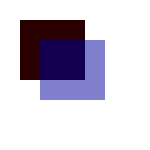
\includegraphics{img/canvas_example1.png}
\caption{Dibuix de dos rectangles superposats amb canvas.}
\label{fig:canvas-exemple-1}
\end{figure} 

L'exemple a continuació s'ha extret\footnote{El codi ha estat simplificat per simplificar la seva comprensió.} d'una pàgina de tutorials sobre canvas\footnote{\url{http://www.html5canvastutorials.com/advanced/html5-canvas-linear-motion-animation/}}. En aquest exemple es descriurà com animar un objecte que s'ha creat dins del canvas, en concret es farà moure un rectangle des de la part esquerra del canvas fins a la seva part dreta. A la mateixa pàgina podeu trobar una demostració de com funciona el codi que es detalla a continuació.

\begin{lstlisting}
window.requestAnimFrame = (function(callback){
    window.setTimeout(callback, 1000 / 60);
})();
 
function animate(lastTime, myRectangle){
    var canvas = document.getElementById("myCanvas");
    var context = canvas.getContext("2d");
 
    // update
    var date = new Date();
    var time = date.getTime();
    var timeDiff = time - lastTime;
    var linearSpeed = 100; // pixels / second
    var linearDistEachFrame = linearSpeed * timeDiff / 1000;
    var currentX = myRectangle.x;
 
    if (currentX < canvas.width - myRectangle.width - myRectangle.borderWidth / 2) {
        var newX = currentX + linearDistEachFrame;
        myRectangle.x = newX;
    }
    lastTime = time;
 
    // clear
    context.clearRect(0, 0, canvas.width, canvas.height);
 
    // draw
    context.beginPath();
    context.rect(myRectangle.x, myRectangle.y, myRectangle.width, myRectangle.height);
 
    context.fillStyle = "#8ED6FF";
    context.fill();
    context.lineWidth = myRectangle.borderWidth;
    context.strokeStyle = "black";
    context.stroke();
 
    // request new frame
    requestAnimFrame(function(){
        animate(lastTime, myRectangle);
    });
}
 
window.onload = function(){
    var myRectangle = {
        x: 0,
        y: 50,
        width: 100,
        height: 50,
        borderWidth: 5
    };
 
    var date = new Date();
    var time = date.getTime();
    animate(time, myRectangle);
};
\end{lstlisting}

En aquestes exemple es creen tres funcions que són les encarregades de realitzar la animació. L'objectiu de cada funció és el següent:

\begin{description}
    \item[requestAnimFrame]{ Encarregat de programar l'execució del pròxim pas de l'animació}
    \item[animate]{ Es l'encarregada de realitzara cada un dels passos de l'animació.}
    \item[window.onload] { Es la funció encarregada d'iniciar l'animació. Com es pot observar l'únic que fa es inicialitzar les variables i cridar a la funció animate per a que dibuixi el primer frame de l'animació.}
\end{description}

De la funció animate (la que s'encarrega de pintar cada un dels frames de l'animació) cal destacar les següents línies:

\begin{description}
    \item[línies 12-22] {Encarregades de calcular el temps que ha passat des de l'ultima execució del codi, per poder saber el nombre de pixels que s'ha de moure l'objecte, tenint en compte que s'utilitza la variable linearSpeed per determinar el nombre de pixels per segons que ha d'abançar l'objecte.}
    \item[línies 25-26] {Netejar tot el conjunt de l'objecte canvas per tal d'esborrar els possibles frames anteriors.}
    \item[línies 28-36] {Encarregades de dibuixar el rectangle a la posició que li toca per al frame actual.}
    \item[línies 38-41] {Crida a la funció requestAnimFrame per programar l'execució del pròxim frame.}
\end{description} 


\section{CSS}

CSS es l'acrònim de \emph{Cascading Style Sheets}, que en català significa "Fulls d'estil en cascada". Els fulls d'estil en cascada s'utilitzen per descriure la semàntica de presentació (l'aspecte i format) d'un document escrit en un llenguatge de marques. La seva aplicació més comuna és dissenyar pàgines web escrites en HTML i XHTML, però el llenguatge també pot ser aplicat a qualsevol classe de document XML, incloent-hi SVG i XUL.

El principal objectiu de CSS és permetre la separació del contingut d'un document escrit amb un llenguatge de marques de la seva presentació. Això permet que múltiples pàgines comparteixin un format comú i també que un mateix document de marcatge es pugui mostrar en diferents formats. En l'àmbit del projecte els fulls d'estil s'utilitzen per definir la presentació del client del projecte.

CSS defineix regles d'estil per a cada element, on s'especifica com es mostrarà cada element. Així també defineix un esquema de prioritat per determinar quines regles d'estil s'apliquen si més d'una regla esta associada amb un element en particular. Aquestes característiques han permès que avui en dia sigui el llenguatge més utilitzat a l'hora de definir l'aspecte i el format d'una pàgina web. 

Tot segut es detallen alguns exemples de codi CSS. 

\begin{lstlisting}
h1 {
    font-family: Arial, sans-serif; 
    font-size: 16px;
    color: red;
}
\end{lstlisting}

L'exemple anterior mostra com aplicar un estil a totes els elements de tipus H1. En aquest cas es defineix que tots elements de tipus H1 s'ha de mostrar amb la font Arial o Sans-serif, han de tenir una mida de lletra de 16px i s'han de mostrar de color roig.  

\begin{lstlisting}
.bordered
{
    border: 1px solid #000;
}
\end{lstlisting}

En l'exemple anterior es declara una classe anomenada \emph{bordered}. La declaració d'una classe ens permet aplicar-la a qualsevol tipus d'element. Per això sol ens cal especificar l'atribut class amb el valor de les classes que volem aplicar. En aquest cas la classe s'utilitza per aplicar una bora de color negre, amb traçat sòlid i d'un píxel de grossor. 

\section{jQuery}

jQuery és una llibreria de Javascript, creada inicial ment per John Resig, que permet simplificar la forma d'interactuar amb els documents HTML, manipular l'arbre DOM, interactuar amb els esdeveniments, desenvolupar animacions i afegir interacció dinàmica a pàgines web. 

jQuery es software de codi obert, llicenciat sota les llicències MIT i LGPLv2. Aquest fet permet que pugui ser usada tan a projectes lliures com a projectes privatius. 

Una de les característiques més interessants de jQuery és que ens permet seleccionar elements de la pàgina a partir de clàusules CSS i aplicar funcions sobre els mateixos. Tot seguit en podem veure alguns exemples: 

\begin{lstlisting}
 jQuery('.bordered').css({'display': 'none'});
\end{lstlisting}

Així el codi anterior el que fa és seleccionar tots els elements de la classe .bordered i modifica les seves propietats CSS per a que no es mostrin a la pàgina. 

\begin{lstlisting}
jQuery('#target').dblclick(function() {
  alert('Handler for .dblclick() called.');
});
\end{lstlisting}

En l'exemple anterior es mostra el codi necessari per associar l'execució d'una funció cada vegada que es produeix un esdeveniment a un object. En concret hem associat una funció que s'executarà cada vegada que es faci doble clic a l'element amb identificar \emph{target}. Aquesta funció simplement mostra un missatge a l'usuari indicant que s'ha produït l'esdeveniment. 

\section{Git}

Git es un sistema de control de versions dissenyat per Linus Torvalds, creador de Linux. Un sistema de control de versions s'encarrega de gestionar els diferents canvis que s'han realitzat sobre un conjunt de fitxers. Una versió o revisió és l'estat en que es troben el conjunts de fitxers en un moment donat en el temps. L'objectiu del control de versions es poder disposar del registre de canvis que s'han realitzat sobre el conjunt de fitxers, permeten saber en quina versió o revisió és trobaven aquell conjunt de fitxers en un moment del passat i quines són les modificacions que els hi hem realitzat. Els sistemes de control de versions permeten que un conjunt de persones puguin realitzar modificacions a la vegada sobre el mateix conjunt de fitxers i ens proporcionen les eines suficients per saber si s'han realitzat modificacions sobre els fitxers i qui les ha realitzat. 

Tot seguit us nombrem les característiques que diferencien Git respecte a altres sistemes de control de versions.

\begin{description}
    \item[Suport per desenvolupament no lineal] Git està dissenyat per tal de proporcionar una interfície ràpida per a crear branques i mesclar-les.
    \item[Distribuït] Cada usuari té un repositori propi. Aquests respositoris poden ser fusionats amb respositoris d'altres usuaris.
    \item[Compatibilitat amb protocols existents] Els respositoris poden ser publicats mitjançant protocols HTTP, FTP, Rsync i fins i tot un protocol propi.
    \item[Eficient per grans projectes] Git es ràpid i escalable. A més a més no es fa més lent a mesura que la història del projecte es fa gran, com passa amb altres sistemes.
    \item[Portable] Funciona tan en sistemes Linux, Unix, MAC i Windows.
\end{description}

Git s'utilitza per controlar totes les modificacions que s'han realitzat al projecte, i perquè altres desenvolupadors interessats en el projecte puguin comunicar-nos modificacions sobre el mateix. A més a més, també ens permet publicar diferents versions del projecte i saber en qualsevol moment quin era l'estat del projecte quan es va publicar una versió. 


\section{Mocha i jscoverage}
\label{sec:mocha-jscoverage}

Mocha\footnote{\url{http://visionmedia.github.com/mocha/}} és una llibreria que s'encarrega d'executar jocs de prova i que funciona sobre el framework node. Aquesta llibreria s'encarrega de detectar quins dels nostres testos estan fallant i reportar-nos els errors a través de diferents formats. Una de les aplicacions més interessant de Mocha és la generació de informes de coverage. Un informe de coverage ens permet visualitzar quines són línies de codi de l'aplicació són executades per un joc de proves i quines no. Per a la generació d'aquest informes es requereix tenir instal·lada la llibreria jscoverage\footnote{\url{http://siliconforks.com/jscoverage/}}. 

En l'àmbit del projecte Mocha s'utiltiza per avaluar els jocs de proves del projecte i validar que tots funcionen correctament. jscoverage s'utilitza per generar un informe que ens permet avaluar quines línies de codi estan sotmeses a jocs de proves i quines no.

\subsection{Formats dels jocs de prova}
\label{sec:format-jocs-prova}
Mocha entén jocs de proves que estan escrits amb els següents formats: BDD, TDD, Exports. Tots seguit es mostra un exemple de cadascun d'ells. 

\subsubsection{BDD}
\begin{lstlisting}
describe('Array', function(){
  before(function(){
    // ...
  });

  describe('#indexOf()', function(){
    it('should return -1 when not present', function(){
      [1,2,3].indexOf(4).should.equal(-1);
    });
  });
});
\end{lstlisting}

En BDD s'utiltizen les función describe(), it(), before(), beforeEach(), after() i aferterEach() per descriure la funcionalitat que es vol implementar i escriure el codi que l'ha de validar.

\subsubsection{TDD}
\begin{lstlisting}
suite('Array', function(){
  setup(function(){
    // ...
  });

  suite('#indexOf()', function(){
    test('should return -1 when not present', function(){
      assert.equal(-1, [1,2,3].indexOf(4));
    });
  });
});

\end{lstlisting}

En TDD s'utiltizen les funcions suite(), test(), setup(), i teardown() per tal d'escriure el codi que ha de validar el correcte funcionament de les especificacions.

\subsubsection{Exports}
\begin{lstlisting}
module.exports = {
  before: function(){
    // ...
  },

  'Array': {
    '#indexOf()': {
      'should return -1 when not present': function(){
        [1,2,3].indexOf(4).should.equal(-1);
      }
    }
  }
};

\end{lstlisting}

El format exports és molt semblant al format utilitzat pel pare de Mocha, expresso. En aquest format es defineix un diccionari on cada objecte és un conjunts de proves i cada funció és un joc de proves. Les claus dels objectes s'utilitzen per especificar el nom del joc de proves. Els noms before, after, beforeEach, i afterEach tenen una connotació especial. 

Durant el transcurs del projecte s'ha utilitzat el format \emph{Exports}, ja que al principi del projecte s'utilitzava expresso per executar els jocs de proves. Així, quan es va migrar a Mocha ja hi havia jocs de proves escrits amb el format \emph{Exports} i es va decidir continuar amb el mateix format per tal d'evitar migrar tots els jocs de proves existents a un nou format. 

\section{JSON}
\label{sec:json}

JSON (acrònim de JavaScript Object Notation) és un estàndard obert basat en text dissenyat per a intercanvi de dades llegible per humans. Deriva del llenguatge script JavaScript, per a representar estructures de dades simples i llistes associatives, anomenades objectes. Malgrat la seva relació amb el JavaScript, té implementacions per a gran part dels llenguatges de programació, alguns exemples són: ActionScript, C, C++, C\#, ColdFusion, Common Lisp, Delphi, E, Eiffel, Java, JavaScript, ML, Objective CAML, Perl, PHP, Python, Rebol, Ruby, Lua y Visual FoxPro. 

El format JSON s'utilitza habitualment per serialitzar i transmetre dades estructurades en una connexió de marxa. S'utilitza principalment per intercanviar dades entre un servidor i una aplicació web, sent una alternativa a l'XML\footnote{\url{https://ca.wikipedia.org/wiki/XML}}. Un dels principals avantatges de JSON respecte a XML és que el primer pot ser directament interpretat amb Javascript i el segon necessita ser parsejat. Això, provoca que el codi Javascript necessari per llegir un fitxer JSON sigui molt més reduït que un XML. A part de la reducció de codi, és molt més ràpid llegir un fitxer en JSON que en XML. 

En les següents línies podeu veure una mostra de com s'estructura la informació en format JSON. 

\begin{lstlisting}
 {"menu": {
   "id": "file",
   "value": "File",
   "popup": {
     "menuitem": [
       {"value": "New", "onclick": "CreateNewDoc()"},
       {"value": "Open", "onclick": "OpenDoc()"},
       {"value": "Close", "onclick": "CloseDoc()"}
     ]
   }
 }}
\end{lstlisting}


\section{Jade}

Jade és un motor de plantilles que ens permet simplificar el codi necessari per a realitzar un pàgina en HTML. Jade s'ha utilitzat en el projecte per tal de generar els fitxers HTML que mostrar el servidor. Gràcies a jade s'ha simplificat el desenvolupament i el manteniment dels mateixos. Un dels principals avantatges de Jade ens que ens permet olvidar-nos de que estem utilitzant un llenguatge de marcatge (HTML). A més a més, Jade ens permet la utilització de variables per a què la mateixa plantilla pugui generar diferents sortides en funció de variables. Aquest fet permet la reutilització de codi.

En les següents línies podeu veure un exemple d'una plantilla escrita amb Jade. 

\begin{lstlisting}
doctype 5
html(lang="en")
  head
    title= pageTitle
    script(type='text/javascript')
      if (foo) {
         bar()
      }
  body
    h1 Jade - node template engine
    #container
      p You are amazing
\end{lstlisting}

Tot seguit podeu veure el HTML que ens queda desprès d'aplicar la plantilla. 

\begin{lstlisting}
<!DOCTYPE html>
<html lang="en">
  <head>
    <title>Jade</title>
    <script type="text/javascript">
      if (foo) {
      	bar()
      }
    </script>
  </head>
  <body>
    <h1>Jade - node template engine</h1>
    <div id="container">
      <p>You are amazing</p>
    </div>
  </body>
</html>	
\end{lstlisting}

\section{Pencil Sketching}
\label{sec:pencil sketcing}
Pencil Sketching és una extensió del navegador web Firefox que ens permet dissenyar prototips d'interfícies gràfiques. Aquesta eina s'ha utilitzat per al dissenyar el prototipus de la interfície gràfica que podeu trobar en el capítol \ref{chap:interficie_usuari}. S'ha triat aquesta eina per la seva simplicitat i perquè ens permet exportar els nostres dissenys a diferents formats, com per exemple: HTML, PNG, documents Openoffice.org, documents Word i PDF. Un altre factor per elegir aquesta tecnologia es que funciona amb tots els sistemes operatius on funciona el navegador web Firefox, ja que és una extensió del mateix. A la figura \ref{fig:pencil} es pot observar una captura de pantalla de l'aplicació. 

\begin{figure}[htbp]
\centering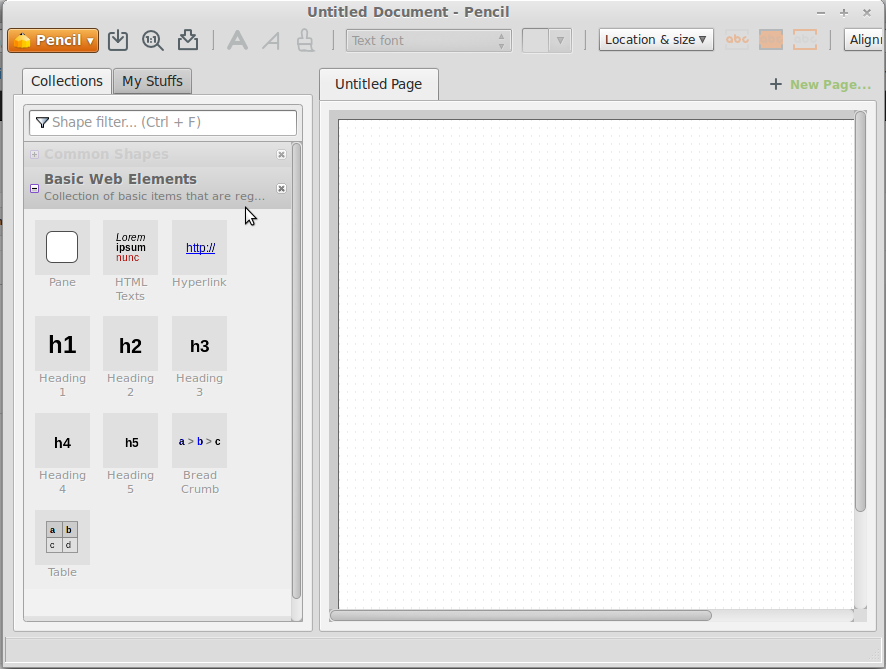
\includegraphics[width=13cm]{img/pencil.png}
\caption{Captura de pantalla de Pencil Sketching.}
\label{fig:pencil}
\end{figure} 


\chapter{Entorn de treball}
%TODO: No m'agrade el nom de entorn de treball -> Buscar alguna cosa més interesant. 

L'Únic requeriment que es necessita per a fer poder fer funcionar el servidor de la botifarra que s'ha implementat es que es disposi del framework node.js instal·lat i instal·lar el paquets dependents del desenvolupament que s'ha realitzat. En aquest apartat s'explicarà com a s'han dut a terme aquestes tasques. 

\section{Instal·lació de node.js}

Actualment per realitzar a instal·lació del Node.js existeixen diferents opcions depenent del sistema operatiu que s'utilitzi: 

\begin{enumerate}
    \item{Autoinstalable per a Windows}
    \item{Autoinstalable per a Mac}
    \item{Repositoris de paquets per a Debian, Ubuntu, OpenSuse, Fedora i derivats i ArchLinux}
    \item{Compilació del codi font}
\end{enumerate}

Quan es va començar a desenvolupar el projecte (Octubre de l'any 2011) no hi havia paquets autoinstalables ni per Mac ni per Windows i els repositoris de paquets de Debian i Ubuntu no estaven actualitzats amb les últimes versions estables de node. De fet Node solament estava suportat sobre sistemes operatius basats en Unix (Mac,Linux,etc.) i no estava suportat per a Sistemes Operatius de Microsoft. 

Per tal de poder disposar de la última versió de node.js es va decidir instal·lar node mitjançant la compilació del codi font. Personalment no soc molt partidari de realitzar instal·lacions a través de compilació de codi font, ja que es bastant engorrós tenir que tornar a compilar tot el codi cada vegada que es publica una nova versió. De totes formes el fet que l'ultima versió estable (en aquells moments la 0.4.x) no estes disponible a través d'un paquet em va fer decidir per la instal·lació a traves de la compilació del codi font. 

\subsection{Requeriments}

La instal·lació de node.js a partir del seu codi font requereix les següent dependències:

\begin{enumerate}
    \item{Python, en la seva versió 2.6 o 2.7. Cal tenir en compte que no podrem instal·lar els paquets des de el codi font si ho intentem des de la versió 3 de Python}
    \item{La llibreria libssl-dev, només en el cas de que es vulgui utilitzar encriptació SSL/TLS. }
\end{enumerate}

\subsection{Obtenció del codi font}

L'obtenció del codi font de la node es pot realitzar de dos formes diferents: 

\begin{enumerate}
    \item{Descarregant un paquet a través de la pàgina oficial de node.js\footnote{\url{http://www.nodejs.org}}}
    \item{Obtenint una copia complerta del respositori de codi font de GitHub\footnote{\url{https://github.com/joyent/node}}}
\end{enumerate}

Així vaig decidir que la millor opció era obtenir una copia del respositori de codi font de GitHub, ja que d'aquesta forma podríem facilitar les actualitzacions: simplement actualitzant el respositori a la última versió i tornant a compilar el codi s'obtindrà la última versió). Una altre motiu per la obtenció del repositori de codi font, es la possibilitat de provar les últimes versions de desenvolupament en el cas de que això fos necessari.  

\subsection{Compilació}

Una vegada s'ha obtingut el codi font aquest pot ser compilat amb les següents comandes:  
\begin{verbatim}
./configure
make
sudo make install
\end{verbatim}

Es pot comprovar que la instal·lació s'ha realitzat de forma correcta teclejant les següent comandes: 

\begin{verbatim}
node
> process.version
\end{verbatim}

Així el programa ens ha de contestar amb la versió que tenim instal·lada, en el meu cas: 'v0.6.7'

\section{Instal·lació de paquets addicionals}

Una de les eines més potents que proporciona node es npm\footnote{Node Package Manager: \url{http://npmjs.org/}}.
Npm s'encarrega de la gestió de mòduls\footnote{Porcions de codi amb una funcionalitat específica, dissenyats per poder ser re-utilitzats} i ens permet utilitzar mòduls publicats per altres desenvolupadors en desenvolupaments propis. També ens permet publicar els nostres propis paquets. 

Inicial ment npm va néixer com una eina separada de node i requeria d'una instal·lació pròpia. A partir de la versió 0.6.0 de node, npm es va integrar a node i s'instal·la de forma automàtica quan es realitza la instal·lació de node. De totes formes npm es pot seguir instal·lant per separat, tal i com es feia a la versions anteriors. La seva instal·lació es pot realitzar amb la següent comanda:

\begin{verbatim}
curl http://npmjs.org/install.sh | sh
\end{verbatim}

Aquesta comanda s'encarrega de baixar d'Internet el codi necessari per a realitzar la instal·lació i d'executar-lo. 

\section{Moduls dependents}

%Explicar com funciona els fitxers packages.json i com nosaltres els fem servir per instal·lar les dependències. 



\chapter{Interfície d'usuari}
\label{chap:interficie_usuari}

La interfície d'usuari és la part que està més exposada al públic de tot el projecte, ja que serà a través d'on els jugadors de la botifarra viuran les seves experiències i interactuaran amb altres jugadors. Per tal de tenir clar des d'un principi com es volia estructurar es va dissenyar una maqueta de la mateixa abans de començar a treballar. 

\section{Maquetes previes}

\begin{figure}[htbp]
\centering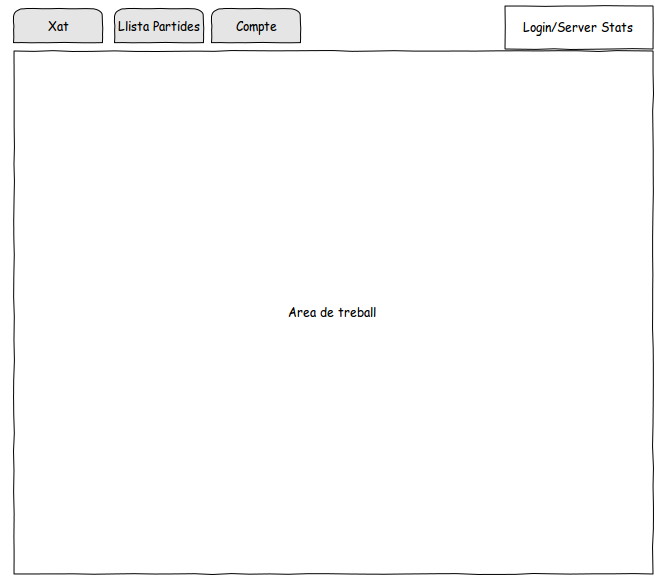
\includegraphics{img/Inici.png}
\caption{Maqueta de la pantalla inicial}
\label{fig:mookup-inici}
\end{figure} 

A la figura \ref{fig:mookup-inici} es pot veure com serà la pantalla inicial. Aquesta s'estructurarà per pestanyes per a que els usuaris puguin accedir a les diferents opcions de la partida. A l'àrea de treball es mostrarà el contingut de les diferents pestanyes. 

\begin{figure}[htbp]
\centering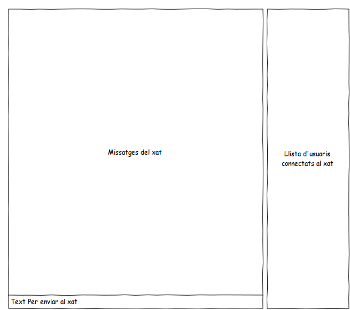
\includegraphics{img/Xat.png}
\caption{Maqueta de la pantalla de Xat}
\label{fig:mookup-xat}
\end{figure} 

A la figura \ref{fig:mookup-xat} es pot veure el contingut que es mostrarà a l'àrea de treball quan la pestanya de xat estigui activa. 

\begin{figure}[htbp]
\centering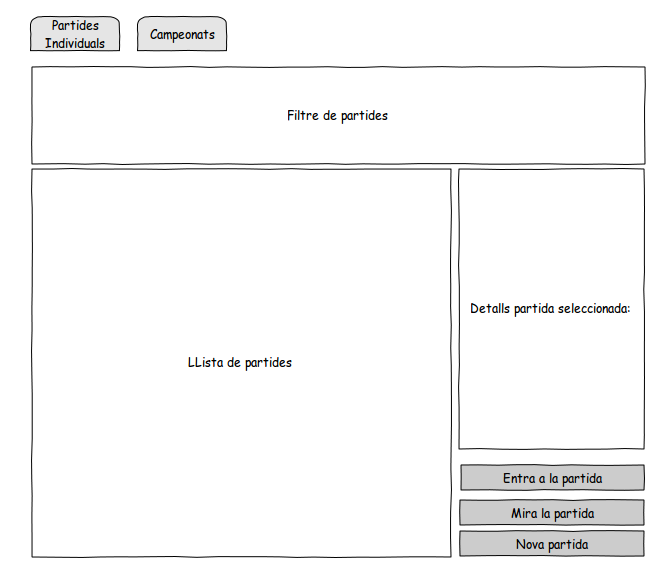
\includegraphics{img/Llista_Partides.png}
\caption{Maqueta del llistat de partides disponibles}
\label{fig:mookup-partides}
\end{figure} 

A la figura \ref{fig:mookup-partides} es pot veure el contingut que es mostrarà a l'àrea de treball quan la pestanya de Llista de partides estigui activa. 

\begin{figure}[htbp]
\centering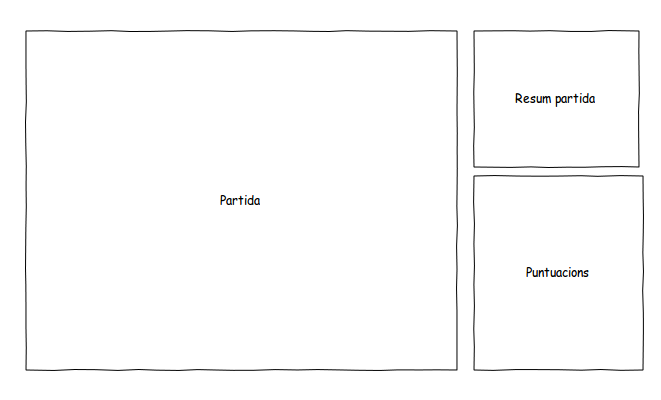
\includegraphics{img/Global_Partida.png}
\caption{Maqueta de la pantalla global de la partida}
\label{fig:mookup-partida}
\end{figure} 

A la figura \ref{fig:mookup-partida} es pot veure el contingut que es mostrarà a l'àrea de treball quan hi hagi una partida en curs. A l'àrea partida serà on els jugadors podran visualitzar el transcurs de la partida i interactuar amb el servidor. Es pot veure en més detall com s'estructura aquesta part en la figura \ref{fig:mookup-detall}.
\begin{figure}[htbp]
\centering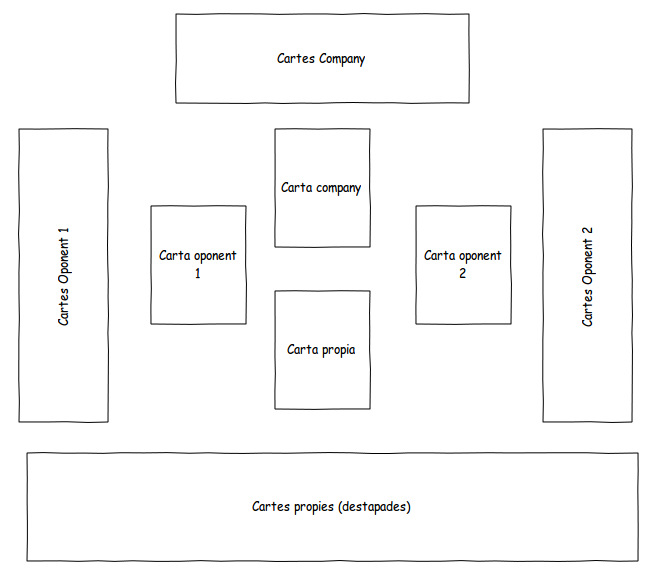
\includegraphics{img/Detall_partida.png}
\caption{Maqueta de la pantalla de detall de la partida}
\label{fig:mookup-detall}
\end{figure} 

\section{Resultat final}

A la figura \ref{fig:real-xat} es pot observar la pantalla que ens mostra l'aplicació després d'identificar-nos. Així al a part equerra podem veure els missatges del xat i a la part dreta la llista d'usuaris que hi ha connectats al servidor. 

\begin{figure}[htbp]
\centering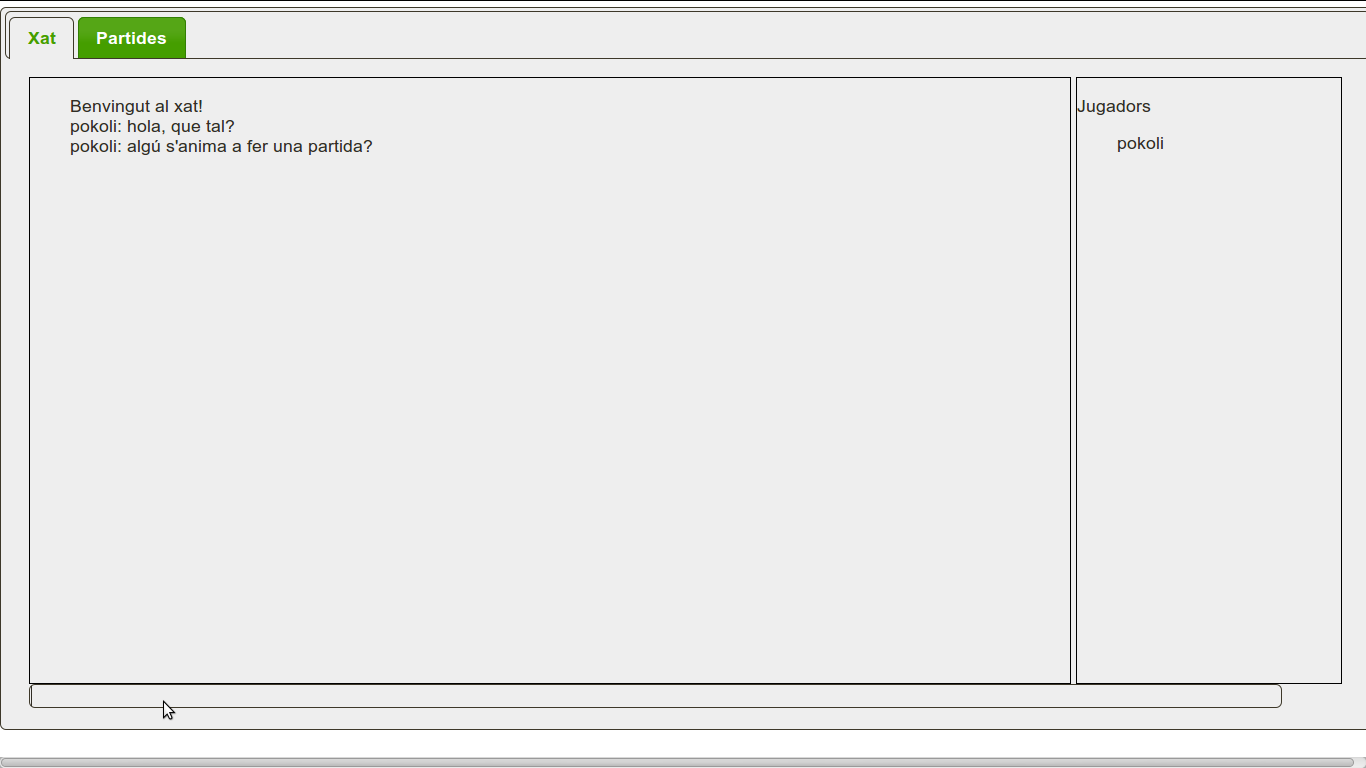
\includegraphics{img/real-xat.png}
\caption{Captura de la pantalla de xat i llista d'usuari.}
\label{fig:real-xat}
\end{figure} 

A la figura \ref{fig:real-partida} es pot veure l'aspecte que té l'aplicació en mitg d'una partida. Així podem veure les nostres cartes, que clicarem per jugar quan sigui el nostre torn, juntament amb les cartes que han jugat els nostres rivals. A la part de la dreta també podem observar les dades generals de la partida, i la puntació de les rondes que s'han jugat fins al moment. 
\begin{figure}[htbp]
\centering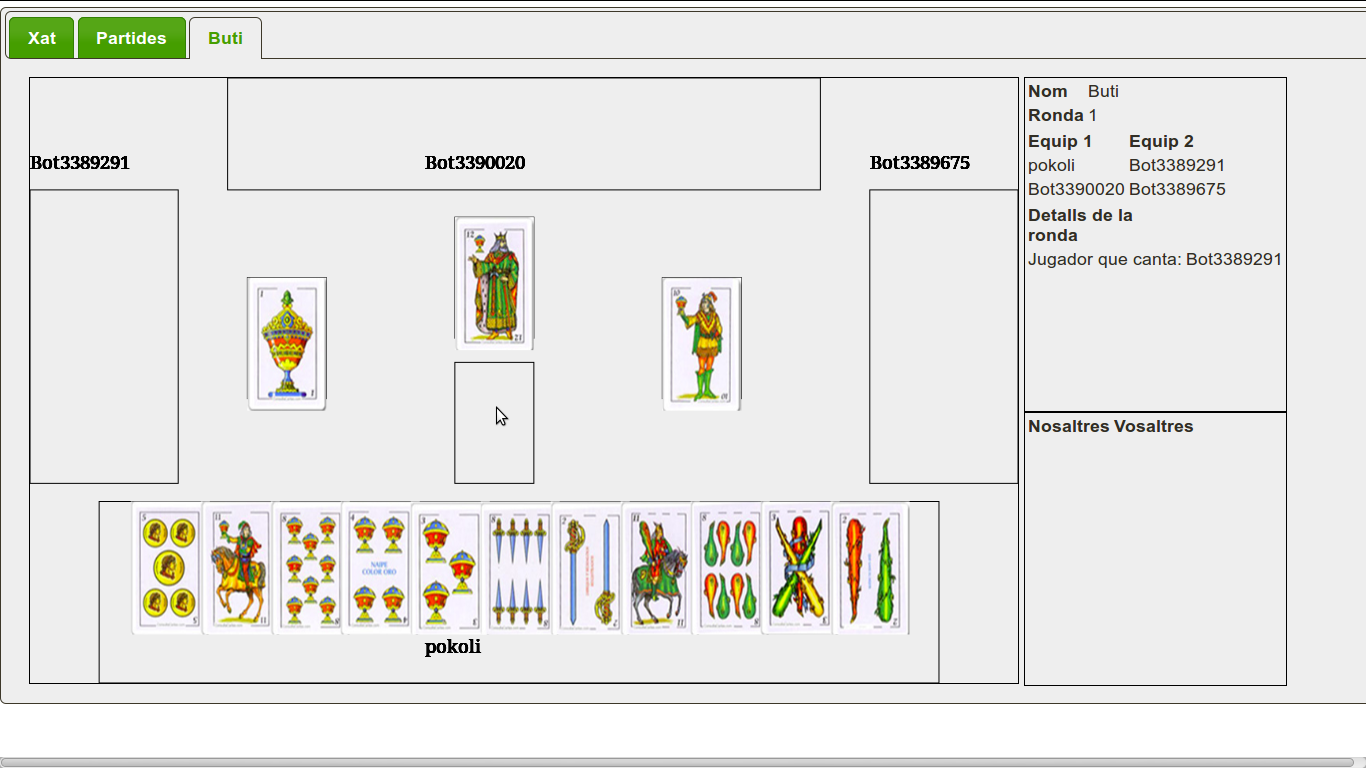
\includegraphics{img/real-partida.png}
\caption{Maqueta de la pantalla de detall de la partida}
\label{fig:real-partida}
\end{figure} 


\end{document}
